\documentclass[a4paper]{article}
\setlength{\parindent}{0pt}

%%%%%%%% CREATE DOCUMENT STRUCTURE %%%%%%%%
%% Language and font encodings
\usepackage[english]{babel}
\usepackage[utf8x]{inputenc}
\usepackage[T1]{fontenc}
%\usepackage{subfig}

%% Sets page size and margins
\usepackage[a4paper,top=3cm,bottom=2cm,left=2cm,right=2cm,marginparwidth=1.75cm]{geometry}

%% Useful packages
\usepackage{framed}
\usepackage{algorithm2e}
\usepackage{amsmath}
\usepackage{graphicx}
%\usepackage[colorinlistoftodos]{todonotes}
\usepackage[colorlinks=true, allcolors=blue]{hyperref}
\usepackage{caption}
\usepackage{subcaption}
\usepackage{listings}
\usepackage{lstautogobble}
\usepackage{sectsty}
\usepackage{apacite}
\usepackage{float}
\usepackage{tikz}
\usepackage{titling} 
\usepackage{blindtext}
\usepackage[square,sort,comma,numbers]{natbib}
\usepackage{xcolor}
\definecolor{darkgreen}{rgb}{0.0, 0.4, 0.0}

\definecolor{pblue}{rgb}{0.13,0.13,1}
\definecolor{pgreen}{rgb}{0,0.5,0}
\definecolor{pred}{rgb}{0.9,0,0}
\definecolor{pgrey}{rgb}{0.46,0.45,0.48}

\usepackage{listings}
\lstset{language=Java,
    showspaces=false,
    showtabs=false,
    breaklines=true,
    showstringspaces=false,
    breakatwhitespace=true,
    commentstyle=\color{pgreen},
    keywordstyle=\color{pblue},
    stringstyle=\color{pred},
    basicstyle=\ttfamily,
    colframe=white!75!black,
    moredelim=[is][\textcolor{pgrey}]{\%\%}{\%\%}
}

\usepackage[most]{tcolorbox}

\newtcblisting{shell}{colback=black,colupper=white,colframe=white!75!black,
	listing only,listing options={language=sh}}

% ToDo: List
\usepackage{enumitem,amssymb}
\newlist{todolist}{itemize}{2}
\setlist[todolist]{label=$\square$}

\usepackage{tikz}
\usetikzlibrary{calc,shapes.multipart,chains,arrows}
\usetikzlibrary{shapes.geometric}
\usetikzlibrary{arrows,shapes,trees}
\usetikzlibrary{calc,shapes.multipart,chains,arrows}
\usetikzlibrary{arrows,shapes}
\usetikzlibrary{arrows.meta, matrix, positioning}
\tikzset{
    queue element/.style={
        draw,very thin,rounded corners,
        fill=yellow!30,
        minimum width=1cm,minimum height=.5cm,
        font=\sffamily\footnotesize
    },
    >={[scale=0.8]Triangle},
    queue/.style={matrix of nodes,
        nodes in empty cells,
        nodes={queue element, anchor=center},
        fill=green!20,
        column sep=5mm,
        row sep=2mm,
    },
}
\tikzstyle{vertex}=[circle,fill=black!25,minimum size=20pt,inner sep=0pt]
\tikzstyle{selected vertex} = [vertex, fill=orange!24]
\tikzstyle{edge} = [draw,thick,-]
\tikzstyle{weight} = [font=\small]
\tikzstyle{selected edge} = [draw,line width=5pt,-,blue!50]
\tikzstyle{ignored edge} = [draw,line width=5pt,-,black!20]
\pgfdeclarelayer{background}
\pgfsetlayers{background,main}


%%%%%%%% DOCUMENT %%%%%%%%
\begin{document}

%%%% Title Page
\begin{titlepage}

\newcommand{\HRule}{\rule{\linewidth}{0.5mm}} 							% horizontal line and its thickness
\center 
% University
\textsc{\LARGE University of Illinois @ Urbana-Champaign}\\[1cm]

% Document info
\textsc{\Large CI 487: Data Structures for CS Teachers}\\[0.2cm]
\textsc{\large }\\[1cm] 										% Course Code
\HRule \\[0.8cm]
{ \huge \bfseries Implementation \#7:\\\vspace{0.1cm}Dijkstra's Shortest Path Algorithm and Prim's Minimum Spanning Tree}\\[0.7cm]								% Assignment
\HRule \\[0.8cm]
\vfill
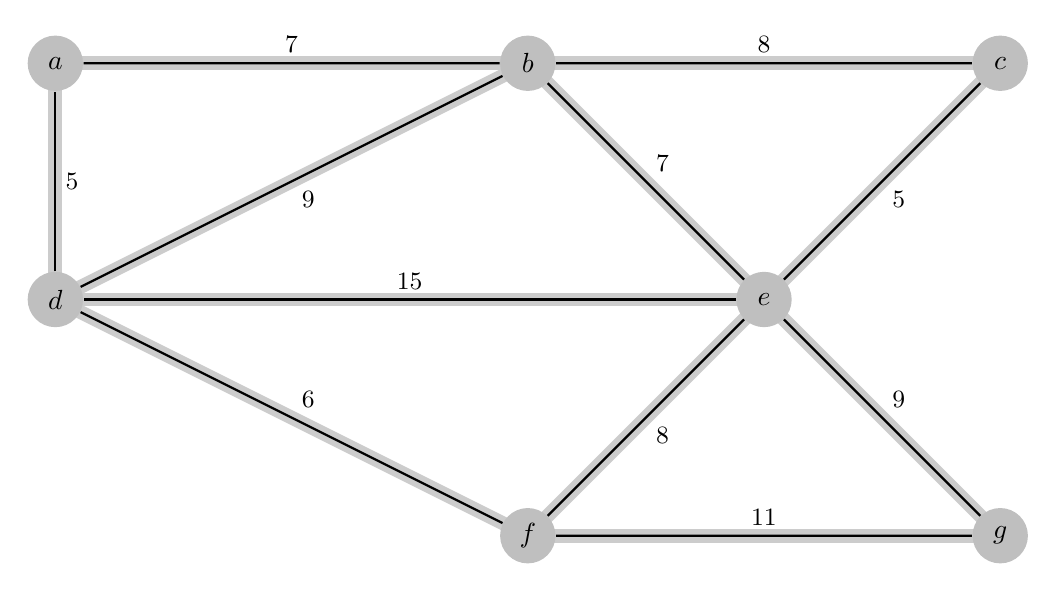
\begin{tikzpicture}[scale=3, auto,swap]
    % Draw a 7,11 network
    % First we draw the vertices
    \foreach \pos/\name in {{(0,1)/a}, {(2,1)/b}, {(4,1)/c},
                            {(0,0)/d}, {(3,0)/e}, {(2,-1)/f}, {(4,-1)/g}}
        \node[vertex] (\name) at \pos {$\name$};
    \foreach \source/ \dest /\weight in {b/a/7, c/b/8,d/a/5,d/b/9,
                                         e/b/7, e/c/5,e/d/15,
                                         f/d/6,f/e/8,
                                         g/e/9,g/f/11}
        \path[edge] (\source) -- node[weight] {$\weight$} (\dest);
    \begin{pgfonlayer}{background}
        \foreach \source / \dest in {d/a,d/f,a/b,b/e,e/c,e/g}
            \path<+->[ignored edge] (\source.center) -- (\dest.center);
        \foreach \source / \dest / \fr in {d/b/4,d/e/5,e/f/5,b/c/6,f/g/7}
            \path<\fr->[ignored edge] (\source.center) -- (\dest.center);
    \end{pgfonlayer}
\end{tikzpicture}
\vfill
\caption{Prim's Minimum Spannning Tree}

%
\includegraphics[width=0.2\textwidth]{images/uiuclogo.png}\\[1cm] 	% University logo
\vfill 
\end{titlepage}

%%%% SECTIONS
%% Section 1
\section{Step 0: The Code You are Given}

To begin, you are given an adjacency list implementation of an undirected,
weighted graph which had the following methods:
\begin{enumerate}
    \item \lstinline|addVertex(E vertex) { ... }|
    \item \lstinline|addEdgeWeighted(E source, E dest, int weight) { ... }|
\end{enumerate}
You can use these methods to create graphs to test your implementations of
Prim's MST and Dijkstra's SP. 

Much like the BST and DFS implementations we will be using extra data 
structures to keep track of attributes related to the state of a given
vertex. For both Dijkstra's and Prim's you are given the same starter code
since both algorithms are tracking the same attributes (i.e., visited, parent,
distance).

\begin{lstlisting}
Map<T, T> parents = new HashMap<T, T>();
Map<T, Integer> dists = new HashMap<>();
Queue<T> pq = new PriorityQueue<T>(Comparator.comparing(dists::get));
\end{lstlisting}

These have the following purposes:
\begin{itemize}
    \item \lstinline|parents|: This keeps track of our vertex's parent by having vertices of type \lstinline|E| as both keys and values.
    \item \lstinline|dists|: This keeps track of the distance attribute related to a given node by having vertices of type \lstinline|E| as keys and \lstinline|Integers| as values.
    \item \lstinline|pq|: This is our min priority queue (lowest value in front) and how we keep track of and access vertices that we still have left to visit. Additionally, we are overriding it's comparison behavior by saying it should get each vertex's value from \lstinline|dists| in order to determine it's position within the priority queue. 
\end{itemize}

Additionally, you are given an implementation of \lstinline|reprioritize| which
removes and readds and entry to a priority queue in order to force said vertex
to be reordered within a priority queue.  This method will appear in the
psudeocode for each of the algorithms and should be called after updating the 
distance attribute associated with a given vertex to ensure it is repositioned 
properly.

\newpage
\subsection{Prim's Minimum-Spanning Tree}
\begin{minipage}{0.54\textwidth}
\RestyleAlgo{ruled} 
\begin{algorithm}[H]
    \caption{Prim's Minimum Spanning Tree}\label{alg:prim}
    \DontPrintSemicolon
    \SetKwFunction{FPrims}{Prim}
    \SetKwProg{Fn}{Function}{}{\KwRet}
    \Fn{\FPrims{G, Source}}{
        \For{ u $\in$ G.Vertecies}{
            u.dist  $\gets \infty$\;
            u.parent $\gets$ null\;
        }
        Source.dist $\gets$ 0\;
        PQ $\gets \emptyset$ \;
        PQ.Enqueue(\textit{all vertecies})\;
        \While{PQ $\neq \emptyset$}{
            u $\gets$ PQ.RemoveMin()\;
            \For{edge $\in$ G.Adj[u]}{
                v $\gets$ eedge.dest\;
                \eIf{v $\in$ PQ AND edge.weight < v.dist}{
                    v.parent $\gets$ u\;
                    v.dist $\gets$ e.weight\;
                    PQ.Reprioritize(v)\;
                }
            }
        }
    }
\end{algorithm}
\end{minipage}
\hfill
% NOTE: Credit for this goes to -> https://texample.net/tikz/examples/prims-algorithm/
\begin{minipage}{0.45\textwidth}
\begin{figure}[H]
\centering
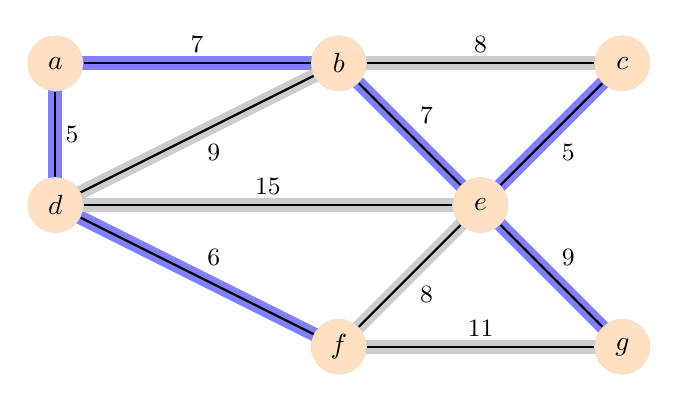
\begin{tikzpicture}[scale=1.8, auto,swap]
    % Draw a 7,11 network
    % First we draw the vertices
    \foreach \pos/\name in {{(0,1)/a}, {(2,1)/b}, {(4,1)/c},
                            {(0,0)/d}, {(3,0)/e}, {(2,-1)/f}, {(4,-1)/g}}
        \node[vertex] (\name) at \pos {$\name$};
    % Connect vertices with edges and draw weights
    \foreach \source/ \dest /\weight in {b/a/7, c/b/8,d/a/5,d/b/9,
                                         e/b/7, e/c/5,e/d/15,
                                         f/d/6,f/e/8,
                                         g/e/9,g/f/11}
        \path[edge] (\source) -- node[weight] {$\weight$} (\dest);
    % Start animating the vertex and edge selection. 
    \foreach \vertex / \fr in {d/1,a/2,f/3,b/4,e/5,c/6,g/7}
        \path<\fr-> node[selected vertex] at (\vertex) {$\vertex$};
    % For convenience we use a background layer to highlight edges
    % This way we don't have to worry about the highlighting covering
    % weight labels. 
    \begin{pgfonlayer}{background}
        \pause
        \foreach \source / \dest in {d/a,d/f,a/b,b/e,e/c,e/g}
            \path<+->[selected edge] (\source.center) -- (\dest.center);
        \foreach \source / \dest / \fr in {d/b/4,d/e/5,e/f/5,b/c/6,f/g/7}
            \path<\fr->[ignored edge] (\source.center) -- (\dest.center);
    \end{pgfonlayer}
\end{tikzpicture}
\caption{Prim's Minimum Spannning Tree (Source = D)}
\end{figure}
\end{minipage}
~\\
For the method \lstinline|primsMST| you should implement the algorithm
described by Algorithm~\ref{alg:prim}. Additionally, after running the 
algorithm your method should print all of the edges that make up the 
minimum spanning tree. Additionally, the following methods may be useful
when implementing this algorithm:
\begin{itemize}
    \item \lstinline|contains(E e)|: The \lstinline|Queue<E>| interface contains a queue method that can be used to determine if the queue contains an element.
    \item \lstinline|offer(E e)|: The \lstinline|Queue<E>| interface uses the \lstinline|offer| method to allow for the enqueueing of elements.
    \item \lstinline|poll(E e)|: The \lstinline|Queue<E>| interface uses the \lstinline|offer| method to allow for the dequeueing of elements.
    \item \lstinline|keySet()|: The \lstinline|Map<E>| interface has this method which will let you get all the keys from a map. For our adjacency graph, the keys are our set of vertecies. This will be useful for when you initially add all vertecies to the queue.
\end{itemize}

\textit{Hint:} After running this algorithm, the \lstinline|parents| HashMap
will contain these edges.

\subsubsection*{Example Output}

\begin{shell}
Prims Edges (Source=D):
A, D
B, A
C, E
D, null
E, B
F, D
G, E
\end{shell}


\newpage
\subsection{Dijkstras Shortest Path Algorithm}

\begin{minipage}{0.53\textwidth}
\RestyleAlgo{ruled} 
\begin{algorithm}[H]
    \caption{Dijkstra's Shortest Path}\label{alg:dijkstra}
    \DontPrintSemicolon
    \SetKwFunction{FDijkstra}{Dijkstra}
    \SetKwProg{Fn}{Function}{}{\KwRet}
    \Fn{\FDijkstra{G, Source, Dest}}{

        \For{ u $\in$ G.Vertex}{
            u.distance  $\gets \infty$\;
            u.parent $\gets$ null\;
        }
        Source.distance $\gets$ 0\;
        PQ $\gets$ G.Vertex\;
        PQ.Enqueue(\textit{all vertecies})\;
        \While{PQ $\neq \emptyset$}{
            u $\gets$ PQ.getMin()\;
            \For{edge $\in$ G.Adj[u]}{
                v $\gets$ edge.dest\;
                PathWeight $\gets$ u.distance + edge.weight)\;
                \If{v $\in$ PQ AND PathWeight < v.distance}{
                    v.parent $\gets$ u\;
                    v.distance $\gets$ PathWeight\;
                    PQ.reprioitize(v)
                }
            }
        }
    }
\end{algorithm}
\end{minipage}
\hfill
% NOTE: Credit for this goes to -> https://texample.net/tikz/examples/prims-algorithm/
\begin{minipage}{0.5\textwidth}
\begin{figure}[H]
\centering
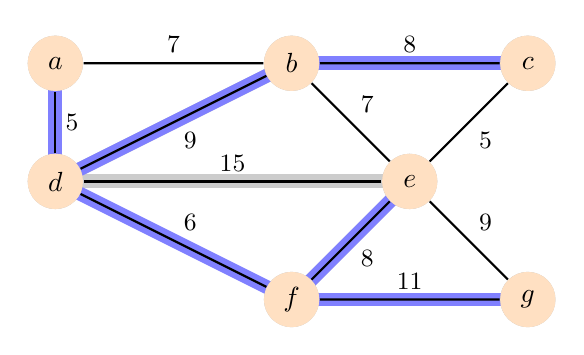
\begin{tikzpicture}[scale=1.5, auto,swap]
    % Draw a 7,11 network
    % First we draw the vertices
    \foreach \pos/\name in {{(0,1)/a}, {(2,1)/b}, {(4,1)/c},
                            {(0,0)/d}, {(3,0)/e}, {(2,-1)/f}, {(4,-1)/g}}
        \node[vertex] (\name) at \pos {$\name$};
    % Connect vertices with edges and draw weights
    \foreach \source/ \dest /\weight in {b/a/7, c/b/8,d/a/5,d/b/9,
                                         e/b/7, e/c/5,e/d/15,
                                         f/d/6,f/e/8,
                                         g/e/9,g/f/11}
        \path[edge] (\source) -- node[weight] {$\weight$} (\dest);
    % Start animating the vertex and edge selection. 
    \foreach \vertex / \fr in {d/1,a/2,f/3,b/4,e/5,c/6,g/7}
        \path<\fr-> node[selected vertex] at (\vertex) {$\vertex$};
    % For convenience we use a background layer to highlight edges
    % This way we don't have to worry about the highlighting covering
    % weight labels. 
    \begin{pgfonlayer}{background}
        \pause
        \foreach \source / \dest / \fr in {d/b/4,d/e/5,e/f/5,b/c/6,f/g/7}
            \path<\fr->[ignored edge] (\source.center) -- (\dest.center);
        \foreach \source / \dest in {b/d, c/b, d/a, f/e, f/d,g/f}
            \path<+->[selected edge] (\source.center) -- (\dest.center);
    \end{pgfonlayer}
\end{tikzpicture}
\caption{Dijkstra's Shortest Path (Source = D)}
\end{figure}
\end{minipage}
~\\
Though there are several variations to Dijkstra's shortest path algorithm the
one we will be focusing on will be for weighted, undirected graphs. This is in
preparation for the final project which deals with the creation and traversal
of a graph of this type. Additionally, we will be focusing on the
implementation on finding the shortest path from a given source node to a given
destination.  The first step in doing this will be to implement
Algorithm~\ref{alg:dijkstra} wich will find the shortest path from a given
source node to \textit{every} vertex in the graph. 
~\\

\RestyleAlgo{ruled} 
\begin{algorithm}[H]
    \caption{Backtrack Traversal from Dijkstra's}\label{algo:dijkstrabacktrack}
    \DontPrintSemicolon
    \SetKwFunction{FPrintDijkstra}{PrintDijkstraSP}
    \SetKwProg{Fn}{Function}{}{\KwRet}
    \Fn{\FPrintDijkstra{G, Source, Dest}}{

        Q $\gets \emptyset$\;
        curr $\gets$ Dest\;
        \While{Source $\notin$ Q}{
            Q.add(curr)\;
            curr = curr.parent\;
        }


    }
\end{algorithm}

~\\
Upon the completion of running the algorithm you should have two data
structures, one storing all of the nodes and their parents and another storing
the total distance from the source node to each vertex in the graph.  We can
use another algorithm to begin at the destination and backtrack to the source.
Along the way we can collect nodes and recreast the shortest path traversal.
The algorithm for doing so is given by Algorithm~\ref{algo:dijkstrabacktrack}.
Here, you will begin at the destination and work your way backwards through
your traversal (i.e., the parents of each vertex) until you find the source.
Once this is done, output that traversal in addition to the total distance.
The methdod you will implement for doing this is called \lstinline|printSP|
and takes: 1) the source vertex, 2) the destination vertex, 3) the map of
parent-child pairs, and 3) the map of distance-value pairs.

\subsubsection*{Example Output}

\begin{shell}
Dijkstras Edges (Source=D, Dest=G):
[D, F, G]: 17
\end{shell}


\end{document}
